\documentclass[hyperref={pdfpagelabels=false}]{beamer}
\usepackage{CJKutf8}
\usepackage[english]{babel}
\usepackage{xcolor}
\usepackage{lmodern}
\usepackage{amssymb}
\usepackage[makeroom]{cancel} %for crossing symbols
\usepackage{leftindex} %For leftindex, making it possible to have nicely aligned left subscripts
%\usepackage{calligra}
%\DeclareMathAlphabet{\mathcalligra}{T1}{calligra}{m}{n} %For small \mathcal letters
\makeatletter
\DeclareFontEncoding{LS1}{}{}
\DeclareFontSubstitution{LS1}{stix}{m}{n}
\DeclareMathAlphabet{\mathKel}{LS1}{stixscr}{m}{n}
\DeclareMathAlphabet{\mathcal}{LS1}{stixscr}{m}{n}
\usepackage{amsthm}
\usepackage{amsmath}
%\usepackage{mathabx}
\usepackage{stmaryrd}
\usepackage{amsbsy}
\usepackage{dsfont}
\usepackage{mathtools} %für mathclap und coloneqq
%\usepackage{amsbsy}
\usepackage{mleftright} %Distanz zu \left \right weg
\usepackage{tikz-cd}

\usepackage{tabularx} %Automatic line break of tables using X instead c l r
%\usepackage{longtable} %table auf mehreren Seiten
%\usepackage{ltxtable} %Combination of both above
\usepackage{xcolor, colortbl}

%Für die ganzen Diagramme
\usepackage{pgfplots}
\usepackage{graphicx} %Für raisebox, vertical displacement of figures
\usetikzlibrary{decorations.markings, decorations.text,calc,arrows.meta}

\definecolor{Gray}{gray}{0.85}
%\usepackage[style=authortitle-icomp]{biblatex}
%\usepackage[babel,german=guillemets]{csquotes}

\setcounter{tocdepth}{1}
%\setcounter{tocdepth}{5}
%\setcounter{secnumdepth}{4}
%\setcounter{secnumdepth}{5}
\usepackage[backend=biber, style=numeric]{biblatex}
\addbibresource{Literatur.bib}
\newcommand{\footlineextra}[1]{
    \begin{tikzpicture}[remember picture,overlay]
        \node[yshift=2ex,anchor=south west] at (current page.south west) {\usebeamerfont{author in head/foot}\hspace{2ex}#1};
    \end{tikzpicture}
}

\newcommand\insertreferences{}
\setbeamertemplate{footline}{%
  \leavevmode%
  \hbox{%
  \begin{beamercolorbox}[wd=.09\paperwidth, ht=5ex,dp=1ex,center, sep=1.4ex]{author in head/foot}%
    \usebeamerfont{author in head/foot}
		%\vfill
		%Sources
		%\vfill
		Sources
  \end{beamercolorbox}%
  \begin{beamercolorbox}[wd=.91\paperwidth,ht=5ex,dp=1ex,center]{title in head/foot}%
    \usebeamerfont{title in head/foot}
    \insertreferences

  \end{beamercolorbox}
}
}


\title{Classification of neighbourhoods of leaves of singular foliations}   
\subtitle{joint work with Camille Laurent-Gengoux\\(Université de Lorraine)}   
\author{Simon-Raphael Fischer} 
\institute{
\begin{figure}
	\centering
		
\includegraphics[width=.50\textwidth]{NCTS.png}
	\label{fig:NCTS}
\end{figure}
\begin{CJK*}{UTF8}{bkai}國家理論科學研究中心\end{CJK*}\\
National Center for Theoretical Sciences (National Taiwan University)
}
\date{} 
%\date{Le lundi 31 mai 2021} 

% zusaetzlich ist das usepackage{beamerthemeshadow} eingebunden 
%\usepackage{beamerthemeIlmenau}
%\usepackage{beamerthemeshadow}
\usepackage{beamerthemeDarmstadt}

%  \beamersetuncovermixins{\opaqueness<1>{25}}{\opaqueness<2->{15}}
%  sorgt dafuer das die Elemente die erst noch (zukuenftig) kommen 
%  nur schwach angedeutet erscheinen 
\beamersetuncovermixins{\opaqueness<1>{25}}{\opaqueness<2->{15}}
% klappt auch bei Tabellen, wenn teTeX verwendent wird\ldots

\beamertemplatenavigationsymbolsempty %Damit sind die kleinen Navigationssymbole unten weg

%\usesectionheadtemplate{}{}
%\usesubsectionheadtemplate{}{}

\def\be{\begin{equation}}
\def\ee{\end{equation}}
\def\bs{\begin{subequations}}
\def\es{\end{subequations}}
\def\ba#1\ea{\begin{align}#1\end{align}}
\def\bes{\begin{equation*}}
\def\ees{\end{equation*}}
\def\bas#1\eas{\begin{align*}#1\end{align*}}

\AtBeginEnvironment{remark}{%
  \setbeamercolor{block title}{use=example text,fg=black,bg=yellow!75!black}
  \setbeamercolor{block body}{parent=normal text,use=block title example,bg=yellow!10}
}

\renewcommand{\qedsymbol}{}
\theoremstyle{plain}
\newtheorem{conjecture}[theorem]{Conjecture}
\newtheorem{proposition}[theorem]{Proposition}
%\newtheorem{definition}[theorem]{Definition}
\theoremstyle{remark}
\newtheorem*{remark}{Remarks}
\newtheorem*{idea}{Idea}
\newtheorem*{motivation}{Motivation}
\newtheorem*{summary}{Summary}
\newtheorem*{situation}{Situation}
\newtheorem*{lab}{Situation: Lie algebra bundles}
\newtheorem*{question}{Question}
\newtheorem*{fieldredefinition}{Field Redefinition}
\newtheorem*{construction}{Construction}
\newtheorem*{aim}{Aim}
\newtheorem*{BackToTheRoots}{Back to the roots}

\AtBeginEnvironment{BackToTheRoots}{%
  \setbeamercolor{block title}{use=example text,fg=black,bg=pink!75!black}
  \setbeamercolor{block body}{parent=normal text,use=block title example,bg=pink!10}
}
\AtBeginEnvironment{idea}{%
  \setbeamercolor{block title}{use=example text,fg=black,bg=pink!75!black}
  \setbeamercolor{block body}{parent=normal text,use=block title example,bg=pink!10}
}

%\theoremstyle{definition}
%\newtheorem{definition}[theorem]{Definition}
%\newtheorem*{SecondIn}{Second Inequality}

%mathrm mit mathup ersetzen, damit die font passt
\renewcommand\familydefault{\sfdefault} %comment to see the difference
\DeclareMathAlphabet      {\mathup}{OT1}{\familydefault}{m}{n}


\begin{document}


\begin{frame}
\thispagestyle{empty}
\titlepage
\end{frame} 


{
\setbeamertemplate{footline}{}
\begin{frame}
%\frametitle{Table of contents}
%\tableofcontents
\thispagestyle{empty}
\begin{figure}[htbp]
	\centering
		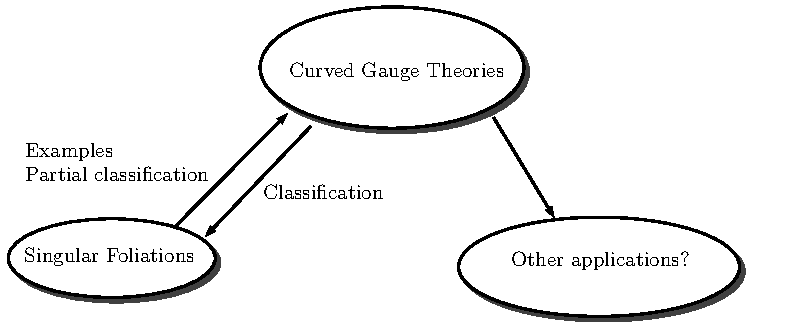
\includegraphics[width=1\textwidth]{Research circles I.pdf}
\end{figure}
\end{frame} 
}

\section{Singular Foliations}

{
\setbeamertemplate{footline}{}
\begin{frame}
\thispagestyle{empty}
\begin{center}
\textbf{\Large Singular Foliations}
\end{center}
\end{frame}
}

{
\setbeamertemplate{footline}
{
  \leavevmode%
  \hbox{%
  \begin{beamercolorbox}[wd=.09\paperwidth,ht=2.25ex,dp=1ex,center]{author in head/foot}%
    \usebeamerfont{author in head/foot}
		Sources
  \end{beamercolorbox}%
  \begin{beamercolorbox}[wd=.91\paperwidth,ht=2.25ex,dp=1ex,center]{title in head/foot}%
    \usebeamerfont{title in head/foot}
		Right diagram made by Mark J.D.\ Hamilton.
  \end{beamercolorbox}%
  %\begin{beamercolorbox}[wd=.175\paperwidth,ht=2.25ex,dp=1ex,right]{date in head/foot}%
    %\usebeamerfont{date in head/foot}\insertshortdate{}\hspace*{2em}
    %%\insertframenumber{} 
		%%/ \inserttotalframenumber\hspace*{2ex} 
  %\end{beamercolorbox}
	}%
  \vskip0pt%
}
\begin{frame}
\begin{tikzpicture}
\coordinate (O) at (0,0);
%\foreach \j in {1,...,3} \draw (O) circle (3.5-\j);
%\foreach \k/\text in {0/Should be here any!,1/There is a way?,2/Wee} \draw[decoration={text along path,reverse path,text align={align=center},text={\text}},decorate] (2.6-\k,0) arc (0:180:2.6-\k);
\foreach \k in {1,...,4}\pgfmathparse{12*\k} \draw[fill=blue!\pgfmathresult] (O) circle (3.6-0.8*\k) node at (0, 3) {$\mathbb{S}^n$};
%\foreach \k/\text in {0/{$S^n$},1/,2/,3/} \draw[decoration={text along path,reverse path,text align={align=center},text={\text}},decorate] (2.9-0.8*\k,0) arc (0:180:2.9-0.8*\k);
\fill (O) circle[radius=2pt];
\begin{scope}[xshift=2.2cm, yshift=-1.8cm]
\begin{axis}[ scale = 1,
            hide axis,
            %axis lines=middle,
%            axis on top,
%            axis line style={blue,dashed,thick},
%            ymin=-2,ymax=2,
%            xmin=-2,xmax=2,
%            zmin=-2,zmax=2,
            samples=40,
            domain=0:360,
            y domain=0:1.25,clip=false
        ]
        \addplot3 [surf, shader=flat, draw=black, fill=gray!10!white, z buffer=sort]
           ({sin(x)*y}, {cos(x)*y}, {(y^2-1)^2});
        \draw[blue,thick,dashed] (axis cs:0,0,0) -- (axis cs:1,0,0)
                    node[below,font=\footnotesize]{};
        \draw[blue,thick,-stealth] (axis cs:1,0,0) -- (axis cs:1.3,0,0)
                    node[above,font=\footnotesize]{};
        \draw[blue,thick,dashed] (axis cs:0,0,0) -- (axis cs:0,-1,0)
                    node[left=2mm,font=\footnotesize]{}; %{Label} am Ende 
        \draw[blue,thick,-stealth] (axis cs:0,-1,0) -- (axis cs:0,-1.5,0)
                    node[right=1mm,font=\footnotesize]{};
        \draw[blue,thick,dashed] (axis cs:0,0,0) -- (axis cs:0,0,1)
                    %node[left=2mm,font=\footnotesize]{$\phi_{\text{RE}}$}
                    ;
        \draw[blue,thick,-stealth] (axis cs:0,0,1) -- (axis cs:0,0,1.3);
\end{axis}
\end{scope}
%\draw[line width=2mm,>={Triangle[length=3mm,width=5mm]},->] (2.6,0) -- (3.8,0);
\end{tikzpicture}
\end{frame}
}

{
\setbeamertemplate{footline}{}
\begin{frame}
\textbf{Singular Foliations:}

\begin{itemize}
	\item Gauge Theory
	\item Poisson Geometry \newline (Singular foliation of symplectic leaves)
	\item Lie groupoids and algebroids
	\item Dirac structures
	\item Generalised complex manifolds
	\item Non-commutative geometry
	\item $\dotsc$
\end{itemize}

\end{frame}
}

\renewcommand\insertreferences{{\tiny  Peter Stefan, Accessible sets, orbits, and foliations with singularities. \textit{Proc.\ London Math.\ Soc.}, 29, 1974.
\newline
Héctor J. Sussmann, Orbits of families of vector fields and integrability of distributions. \textit{Trans.\ Amer.\ Math.\ Soc.}, 180, 1973}}

\subsection{Definition}

\begin{frame}
\begin{definition}[Smooth singular foliation]
A \textbf{smooth singular foliation $\mathcal{F}$} on a smooth manifold is a subspace of $\mathfrak{X}_c(M)$ so that
\begin{itemize}
	\item it is \textbf{involutive},
	\item it is \textbf{stable under $C^\infty(M)$-multiplication},
	\item it is \textbf{locally finitely generated}.
\end{itemize}
\end{definition}
\end{frame}

\begin{frame}
\begin{definition}[Smooth singular foliation]
A \textbf{smooth singular foliation $\mathcal{F}$} on a smooth manifold is a subspace of $\mathfrak{X}_c(M)$ so that
\begin{itemize}
	\item it is \textbf{involutive}, \textit{i.e.\ $[\mathcal{F}, \mathcal{F}] \subset \mathcal{F}$},
	\item it is \textbf{stable under $C^\infty(M)$-multiplication},
	\item it is \textbf{locally finitely generated}.
\end{itemize}
\end{definition}
\end{frame}

\begin{frame}
\begin{definition}[Smooth singular foliation]
A \textbf{smooth singular foliation $\mathcal{F}$} on a smooth manifold is a subspace of $\mathfrak{X}_c(M)$ so that
\begin{itemize}
	\item it is \textbf{involutive}, \textit{i.e.\ $[\mathcal{F}, \mathcal{F}] \subset \mathcal{F}$},
	\item it is \textbf{stable under $C^\infty(M)$-multiplication}, \textit{i.e.\ $fX \in \mathcal{F}$ for all $f \in C^\infty(M)$ and $X \in \mathcal{F}$},
	\item it is \textbf{locally finitely generated}.
\end{itemize}
\end{definition}
\end{frame}

\begin{frame}
\begin{definition}[Smooth singular foliation]
A \textbf{smooth singular foliation $\mathcal{F}$} on a smooth manifold is a subspace of $\mathfrak{X}_c(M)$ so that
\begin{itemize}
	\item it is \textbf{involutive}, \textit{i.e.\ $[\mathcal{F}, \mathcal{F}] \subset \mathcal{F}$},
	\item it is \textbf{stable under $C^\infty(M)$-multiplication}, \textit{i.e.\ $fX \in \mathcal{F}$ for all $f \in C^\infty(M)$ and $X \in \mathcal{F}$},
	\item it is \textbf{locally finitely generated}, \textit{i.e.\ around each $p \in M$ there is an open neighbourhood $U$ and a finite family $\mleft( X^i \mright)_i^{r}$ ($X^i \in \mathcal{F}$) such that for all $X \in \mathcal{F}$ there are $f_i \in C^\infty(M)$ satisfying on $U$}.
	\bas
	X = \sum_i f_i X^i.
	\eas
\end{itemize}
\end{definition}
\end{frame}

\begin{frame}
\begin{remark}[Leaves]
Following the flows in $\mathcal{F}$, this gives rise to a partition of connected immersed submanifolds in $M$.
\end{remark}

\begin{figure}[htbp]
	\centering
		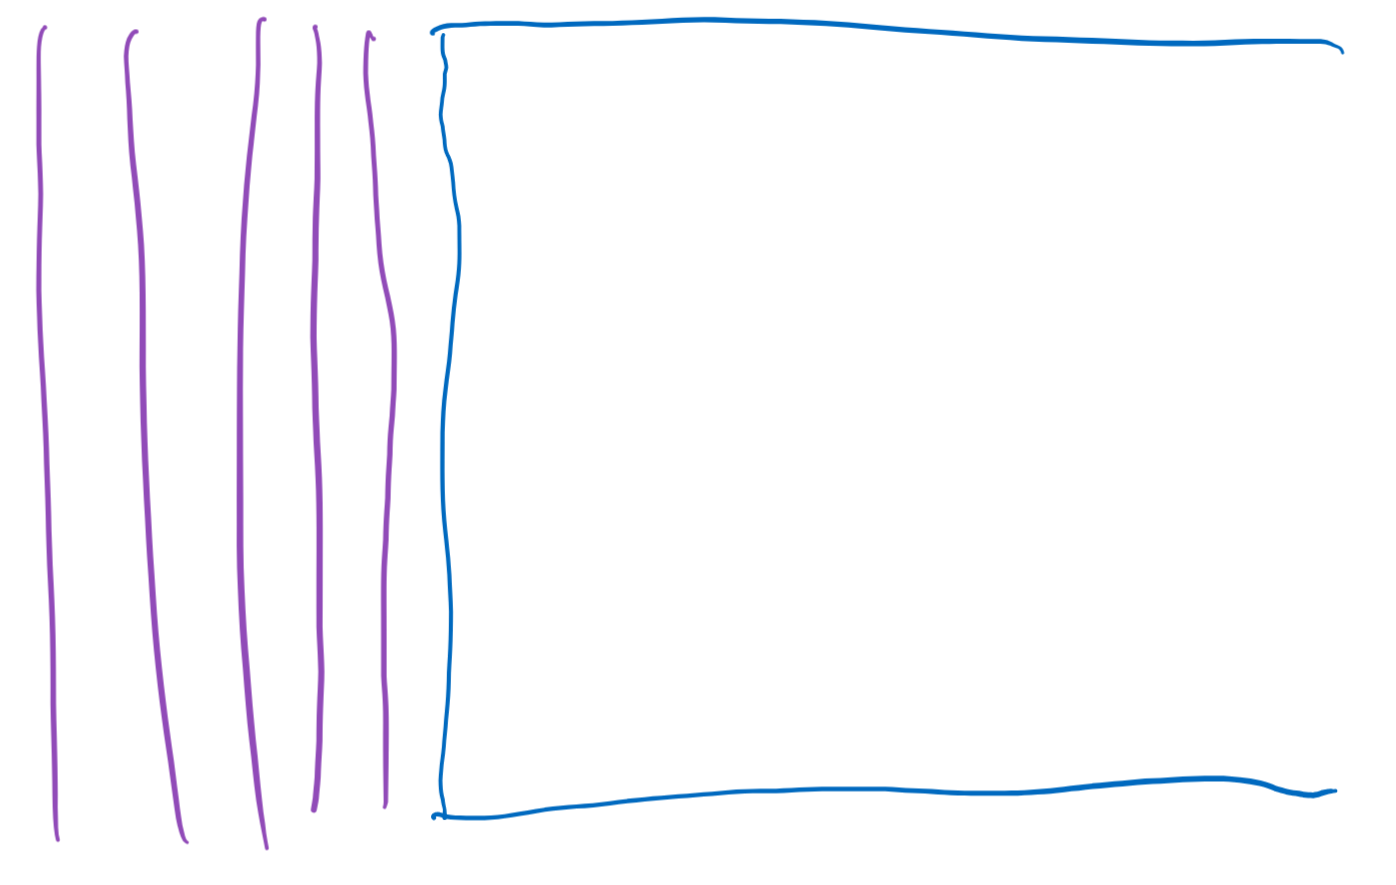
\includegraphics[width=.70\textwidth]{Foliation example.png}
	\label{fig:Foliation example}
\end{figure}


\end{frame}

%{
%\setbeamertemplate{footline}
%{
  %\leavevmode%
  %\hbox{%
  %\begin{beamercolorbox}[wd=.09\paperwidth,ht=2.25ex,dp=1ex,center]{author in head/foot}%
    %\usebeamerfont{author in head/foot}
		%Sources
  %\end{beamercolorbox}%
  %\begin{beamercolorbox}[wd=.91\paperwidth,ht=2.25ex,dp=1ex,center]{title in head/foot}%
    %\usebeamerfont{title in head/foot}
		%Private communication with Camille Laurent-Gengoux.
  %\end{beamercolorbox}%
  %%\begin{beamercolorbox}[wd=.175\paperwidth,ht=2.25ex,dp=1ex,right]{date in head/foot}%
    %%\usebeamerfont{date in head/foot}\insertshortdate{}\hspace*{2em}
    %%%\insertframenumber{} 
		%%%/ \inserttotalframenumber\hspace*{2ex} 
  %%\end{beamercolorbox}
	%}%
  %\vskip0pt%
%}
%\begin{frame}{Why finitely generated?}
%
%\begin{figure}[htbp]
	%\centering
		%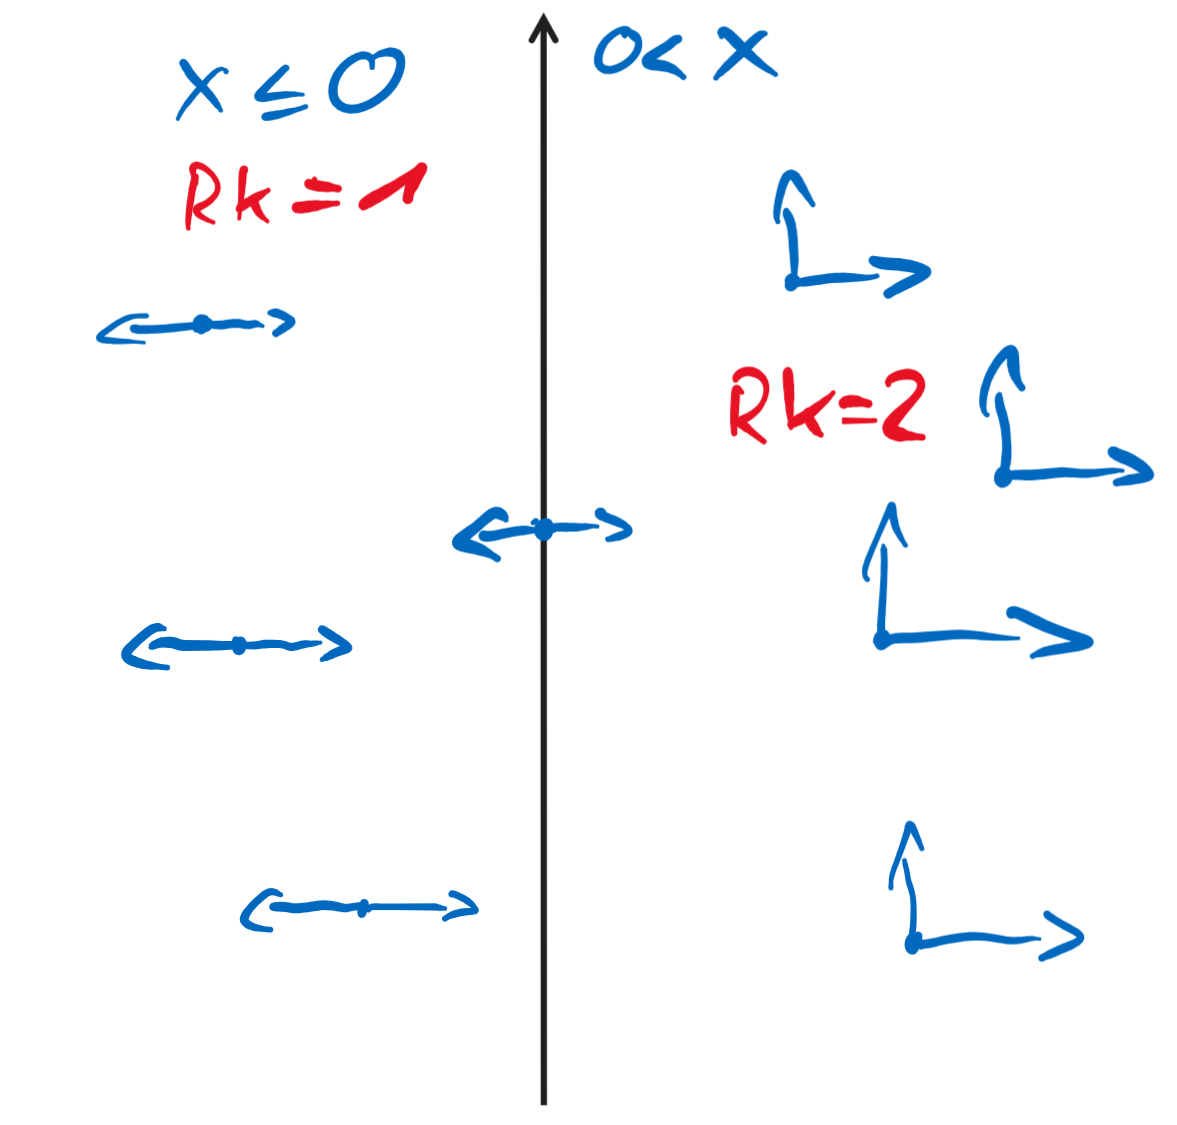
\includegraphics[width=0.50\textwidth]{Infinite comb.png}
	%\caption{Infinite Comb}
	%\label{fig:Infinite comb}
%\end{figure}
%\end{frame}
%}

\subsection{Idea: Relation to gauge theory}

\renewcommand\insertreferences{{\tiny Camille Laurent-Gengoux and Leonid Ryvkin, The holonomy of a singular leaf, \newline \textit{Selecta Mathematica 28}, no.\ 2, 45, 2022.}}

\begin{frame}
\begin{figure}[htbp]
	\centering
		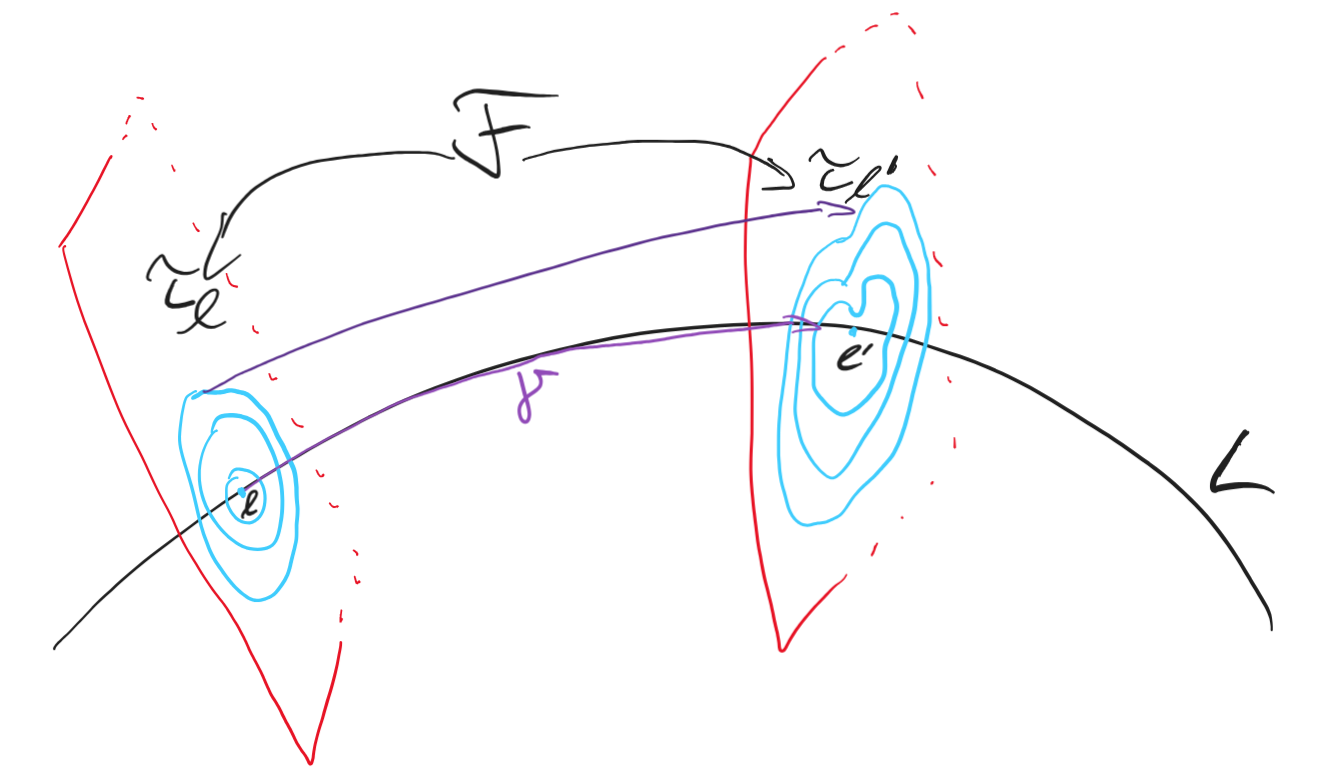
\includegraphics[width=1.00\textwidth]{Foliation connection.png}
	%\caption{$\mathcal{F}$-connections}
	\label{fig:Foliation connection}
\end{figure}

\end{frame}

\begin{frame}
\begin{figure}[htbp]
	\centering
		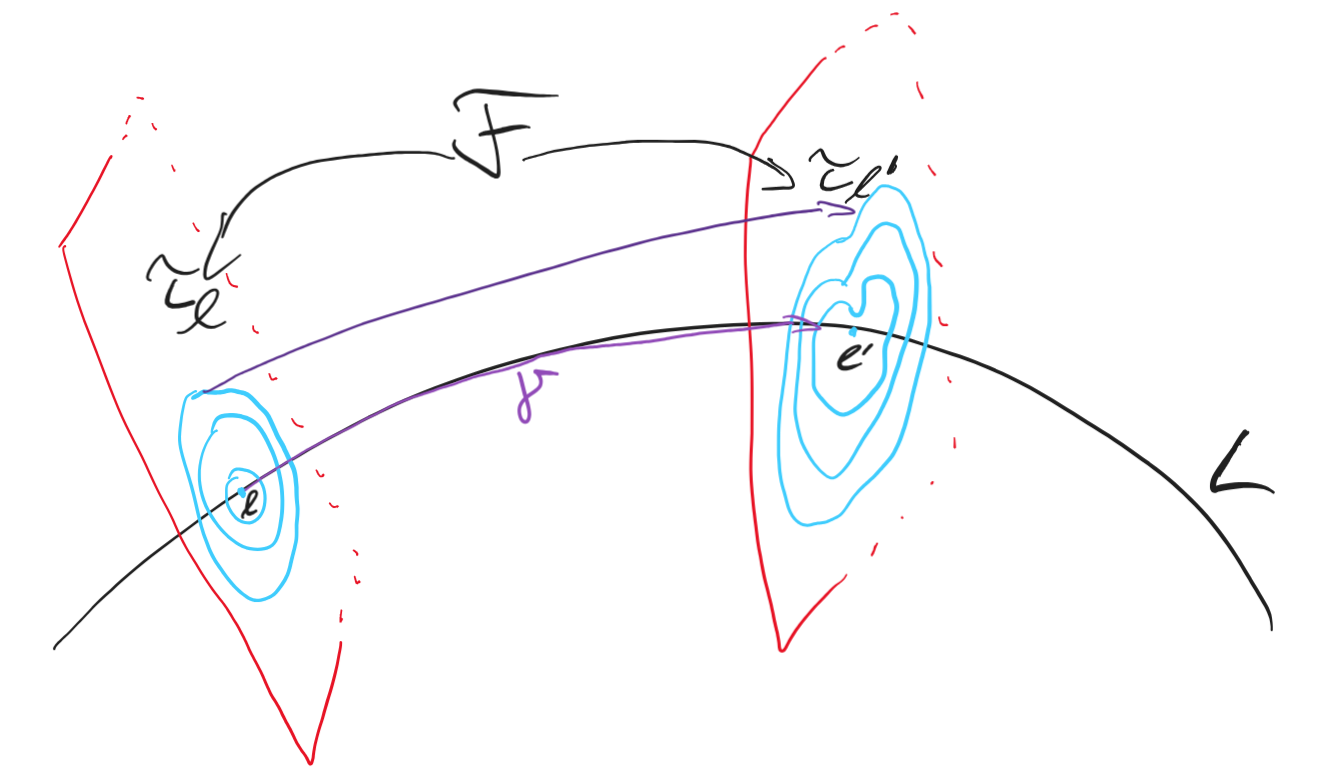
\includegraphics[width=0.50\textwidth]{Foliation connection.png}
	%\caption{$\mathcal{F}$-connections}
	\label{fig:Foliation connection Zwei}
\end{figure}

\begin{theorem}[$\mathcal{F}$-connections]
There is a connection on the normal bundle of a leaf $L$:
\begin{itemize}
	\item Horizontal vector fields are in $\mathcal{F}$.
	\item Parallel transport $\mathup{PT}_\gamma$ has values in $\mathup{Sym}(\tau_l, \tau_{l^\prime})$.
	\item For a contractible loop $\gamma_0$ at $l$: $\mathup{PT}_{\gamma_0}$ values in $\mathup{Inner}(\tau_l)$.
\end{itemize}
\end{theorem}

\end{frame}

\begin{frame}{Example of a transverse foliation $\tau$:}
%\begin{center}
\begin{minipage}[]{0.45\textwidth}
\begin{figure}
\begin{tikzpicture}
\coordinate (O) at (0,0);
\foreach \k in {1,...,4}\pgfmathparse{12*\k} \draw[fill=blue!\pgfmathresult] (O) circle (3.6-0.8*\k) node at (0, 3) {$\mathbb{S}^n$};
\fill (O) circle[radius=2pt];
\end{tikzpicture}
\end{figure}
%\end{center}
\end{minipage}
\hfill
\begin{minipage}[]{0.45\textwidth}
\begin{remark}
\begin{itemize}
	\item $\mathup{Inner}(\tau_l)$ maps each circle to itself
	\item $\mathup{Sym}(\tau_l)$ allows to exchange circles
	\item Both preserve $\tau_l$ and fix the origin
\end{itemize}
\end{remark}
\end{minipage}
\end{frame}

{
\setbeamertemplate{footline}{}

\begin{frame}
\begin{figure}[htbp]
	\centering
		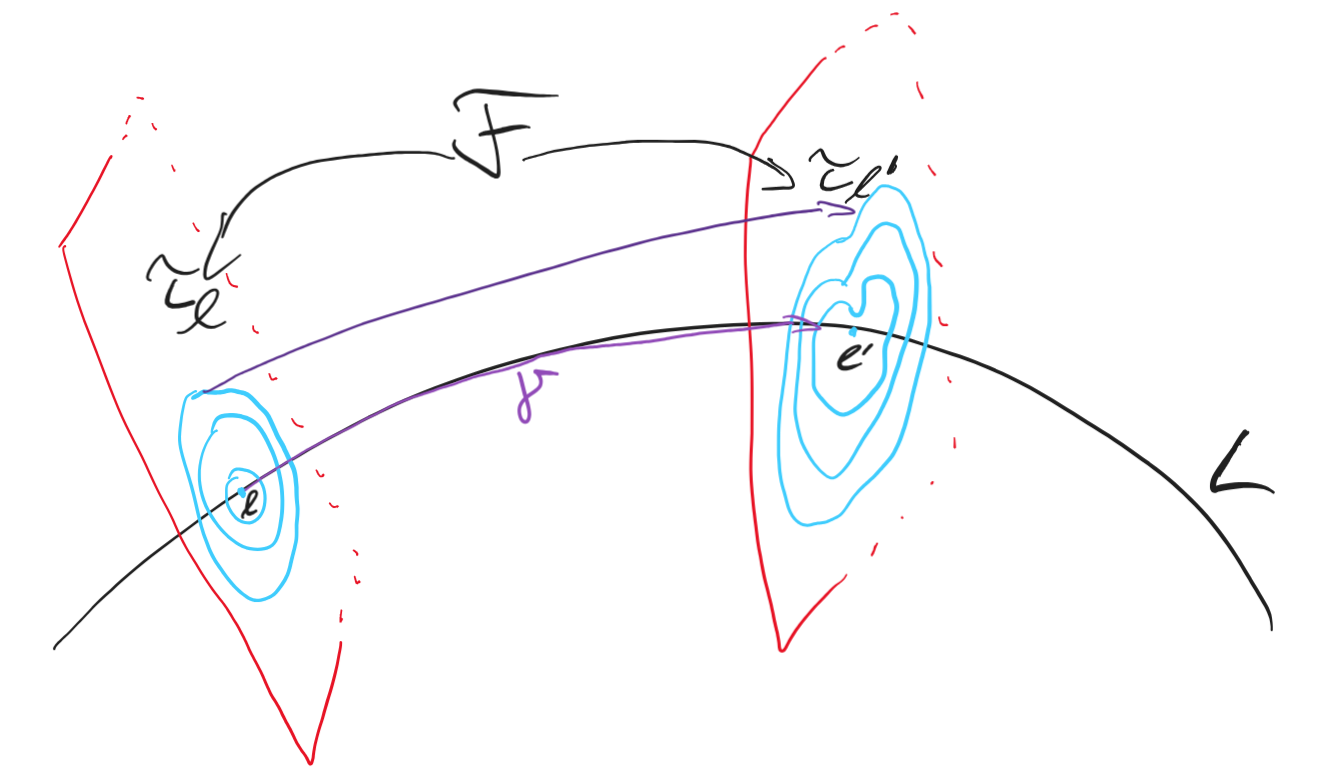
\includegraphics[width=0.4\textwidth]{Foliation connection.png}
	%\caption{$\mathcal{F}$-connections}
	\label{fig:Foliation connection Zwei}
\end{figure}

\begin{remark}[$\mathcal{F}$-connection]
For $\phi \in \mathup{Sym}(\tau_l)$ we have an induced parallel transport
\bas
\mathup{PT}_\gamma^{\mathup{Sym}}(\phi) \coloneqq \mathup{PT}_\gamma \circ \phi \circ \mathup{PT}_\gamma^{-1}.
\eas
Then, on the normal bundle $\pi \colon \mathcal{T} \to L$,
\bas
\mathup{PT}_\gamma(\phi \cdot p)
&=
\mathup{PT}_\gamma^{\mathup{Sym}}(\phi) \cdot
\mathup{PT}_\gamma( p)
\\
\mathup{PT}_{\gamma_0}(p)
&=
\varphi \cdot p
\eas
for all $p \in \mathcal{T}_l$, $\phi \in \mathup{Sym}(\tau_l)$, and
for some $\varphi \in \mathup{Inner}\mleft(\tau_{l}\mright)$.
\end{remark}

\end{frame}

\begin{frame}
\begin{figure}[htbp]
	\centering
		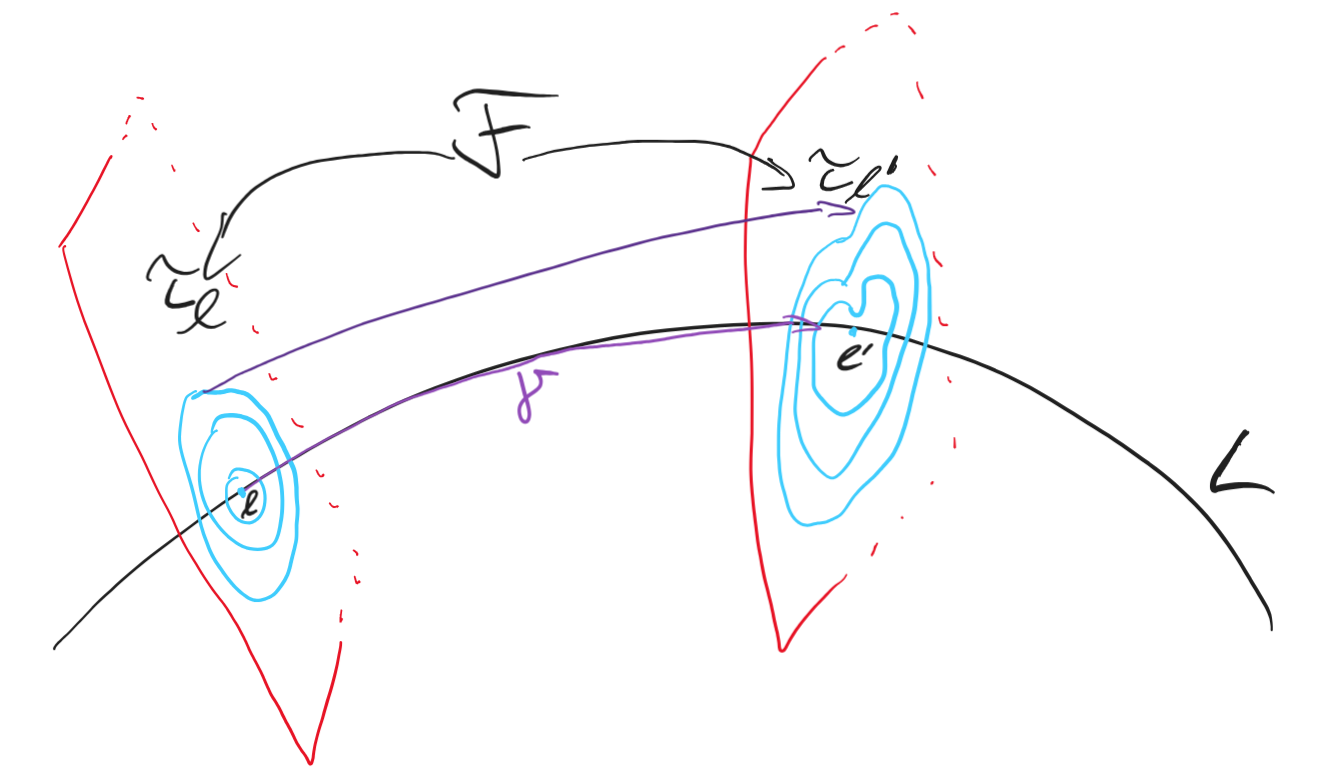
\includegraphics[width=0.4\textwidth]{Foliation connection.png}
	%\caption{$\mathcal{F}$-connections}
	\label{fig:Foliation connection Zwei}
\end{figure}

\begin{remark}[$\mathup{Sym}$-connection]
For $\phi \in \mathup{Sym}(\tau_l)$ we have an induced parallel transport
\bas
\mathup{PT}_\gamma^{\mathup{Sym}}(\phi) \coloneqq \mathup{PT}_\gamma \circ \phi \circ \mathup{PT}_\gamma^{-1}.
\eas
Then
\bas
\mathup{PT}_\gamma(\phi \circ \phi')
&=
\mathup{PT}_\gamma^{\mathup{Sym}}(\phi) \circ
\mathup{PT}_\gamma^{\mathup{Sym}}(\phi')
\\
\mathup{PT}^{\mathup{Sym}}_{\gamma_0}(\phi)
&=
\varphi \circ \phi \circ \varphi^{-1}
\eas
for all $\phi, \phi' \in \mathup{Sym}(\tau_l)$, and
for some $\varphi \in \mathup{Inner}\mleft(\tau_{l}\mright)$.
\end{remark}

\end{frame}

\begin{frame}{Idea}
\begin{figure}[htbp]
	\centering
		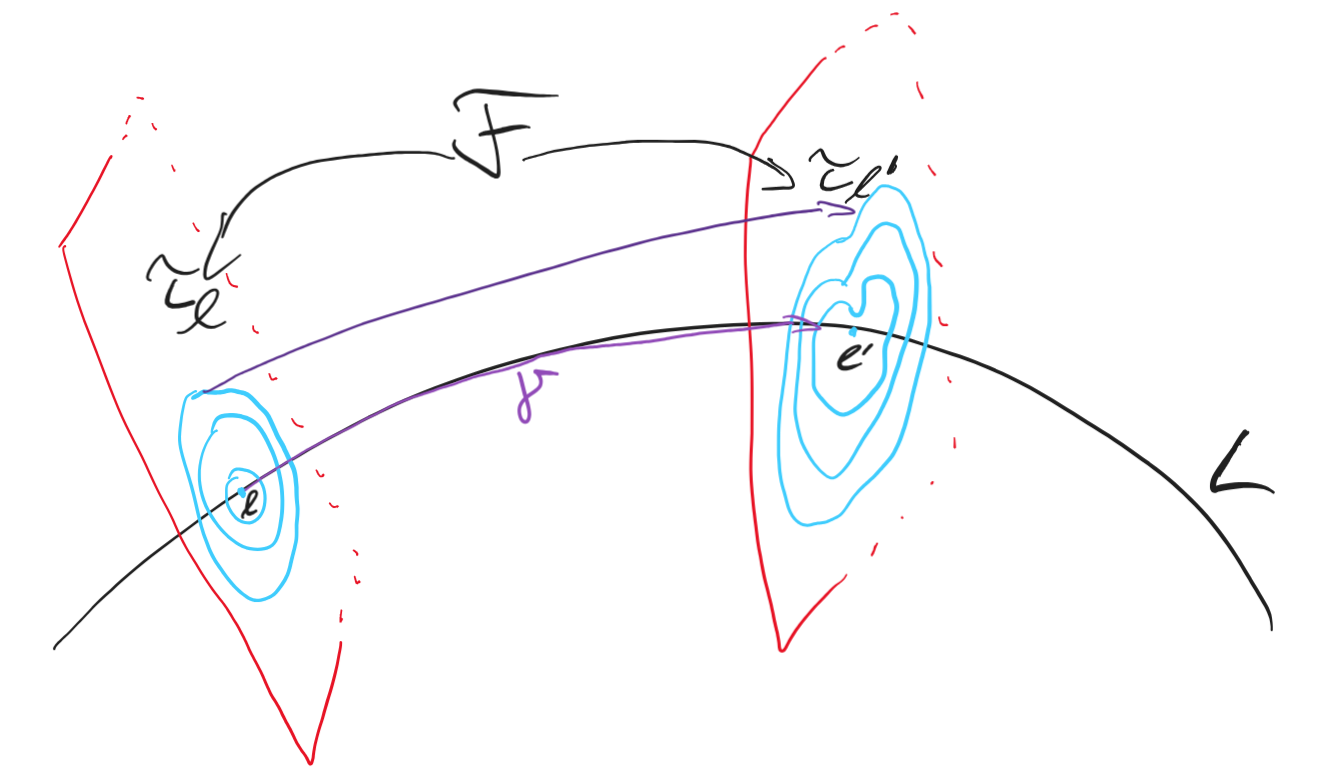
\includegraphics[width=0.5\textwidth]{Foliation connection.png}
	%\caption{$\mathcal{F}$-connections}
	\label{fig:Foliation connection Drei}
\end{figure}

\begin{idea}
Generators of $\mathcal{F}$ given by $\mathcal{F}_{\mathup{projectable}}$:
\bas
\mathbb{H}(X) + \overline{\nu},
\eas
where $X \in \mathfrak{X}(L)$, $\mathbb{H}(X)$ its projectable horizontal lift, $\nu \in \Gamma(\mathrm{inner}(\tau))$ and $\overline{\nu}$ its fundamental vector field.

\end{idea}
\end{frame}

\begin{frame}
\begin{figure}[htbp]
	\centering
		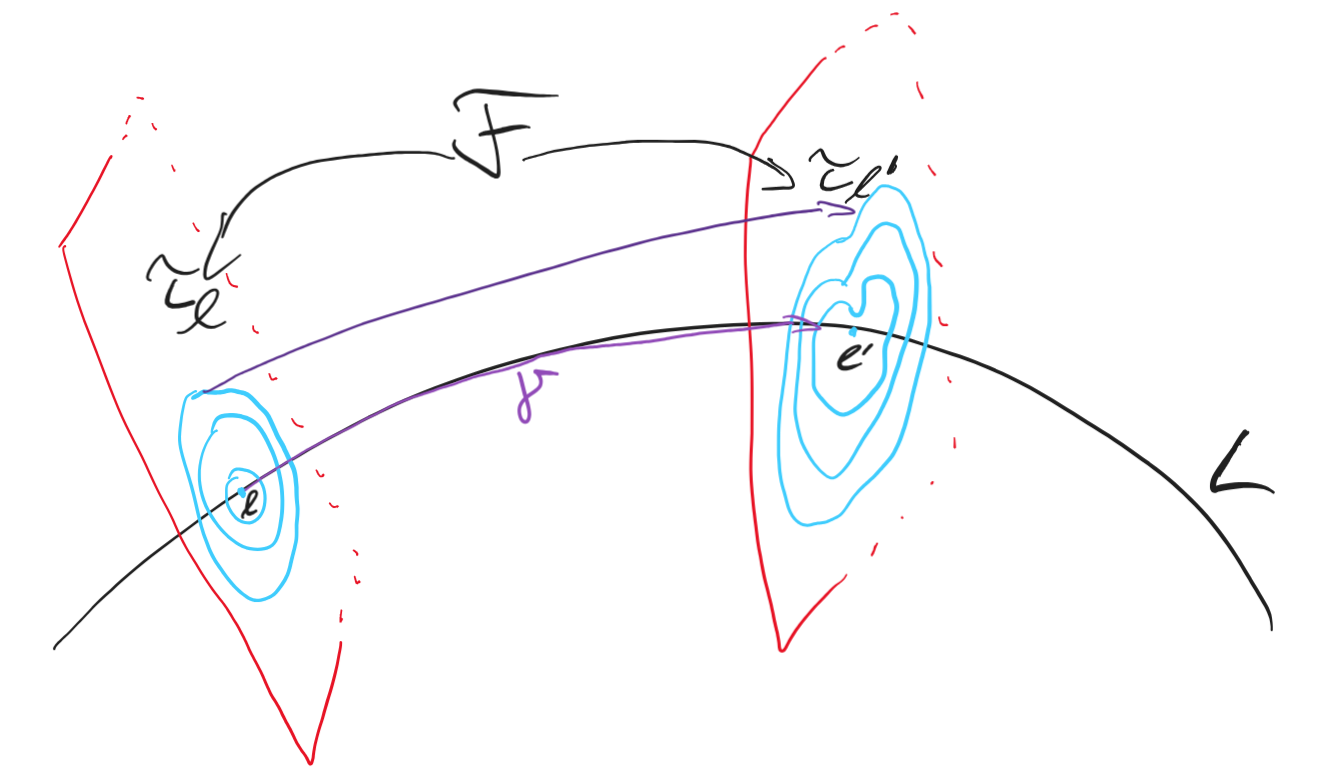
\includegraphics[width=0.5\textwidth]{Foliation connection.png}
	%\caption{$\mathcal{F}$-connections}
	\label{fig:Foliation connection Vier}
\end{figure}
\begin{idea}
Fix $l$ and given $\tau_l$: Reconstruct $\mathcal{F}$.
\bas
\mleft[ \mathbb{H}(X) + \overline{\nu}, \mathbb{H}\mleft({X^\prime}\mright) + \overline{\mu} \mright]
&=
\mathbb{H}\mleft(\mleft[ X, X' \mright]\mright) + 
\overline{\vphantom{d}
\dots
}
\\
&=
\underbrace{\mleft[ \mathbb{H}(X), \mathbb{H}\mleft({X^\prime}\mright) \mright]}_{\rightsquigarrow \text{ curvature}}
\\
&\hspace{1cm}
	+ \underbrace{\mleft[ \mathbb{H}(X), \overline{\mu} \mright]
	- \mleft[ \mathbb{H}\mleft({X^\prime}\mright), \overline{\nu} \mright]}_{\rightsquigarrow \text{ connection}}
	+ \overline{\mleft[ \nu, \mu \mright]}
\eas
\end{idea}
\end{frame}
}

\section{Multiplicative Yang-Mills connections}
\subsection{Lie group bundle actions}
{
\setbeamertemplate{footline}{}

\begin{frame}
\thispagestyle{empty}
\begin{center}
\textbf{\Large Multiplicative Yang-Mills connections}
\end{center}
\end{frame}

\begin{frame}
\textbf{Curved Yang-Mills gauge theories:}
\begin{table}[h!]
	\centering
		\begin{tabular}{c c} 
			%\rowcolor{gray}
			Classical & Curved \\
			%Infinitesimal & Lie algebra $\mathfrak{g}$ & LAB\footnote{LAB = Lie algebra bundle} $\mathcal{g}$ \\
			%\rowcolor{Gray}
			Lie group $G$ & \textcolor[rgb]{1,0.41,0.13}{Lie group bundle
			%\footnote{LGB = Lie group bundle} 
			$\mathcal{G}$}
		\end{tabular}
\end{table}

\begin{center}
	\begin{tikzcd}[ampersand replacement=\&]
	G \arrow{r} \& \mathcal{G} \arrow{d} \\
	\& L
	\end{tikzcd}
\end{center}
\pause
\begin{remark}[Why a "curved theory"?]
Usually, the field strength $F$ is given by (abelian, for simplicity)
\bas
F
&\coloneqq
\mathrm{d}A
=
\mathrm{d}^{\nabla^0}A.
\eas
$\rightsquigarrow$ We will use a general connection $\nabla$ instead of $\nabla^0$, and $\nabla$ may not be flat.
\end{remark}
\end{frame}
}

\renewcommand\insertreferences{{\tiny  K. Mackenzie. General Theory of Lie Groupoids and Algebroids. \newline \textit{London Mathematical Society Lecture Note Series}, 213, 2005.}}

\begin{frame}
\begin{definition}[LGB actions]
\begin{center}
	\begin{tikzcd}[ampersand replacement=\&, column sep = small, row sep = small]
	 \& \mathcal{G} \arrow[bend right]{dl} \arrow{d}{\pi_{\mathcal{G}}} \\
	\mathcal{T} \arrow{r}{\pi} \& L
	\end{tikzcd}
\end{center}
A \textbf{right-action of $\mathcal{G}$ on $\mathcal{T}$} is a smooth map 
%\bas
$\mathcal{T} * \mathcal{G} \coloneqq \mathcal{T} \leftindex^{}_{\pi}\times_{\pi_{\mathcal{G}}} \mathcal{G} \to \mathcal{T}$,
$(p, g) \mapsto p \cdot g$,
%\eas
satisfying the following properties:
\ba\label{InvarianceOffUnderGAction}
\pi(p \cdot g) &= \pi(p),\\
(p \cdot g) \cdot h &= p \cdot (gh),\\
p \cdot e_{\pi(p)} &= p
\ea
for all $p \in \mathcal{T}$ and $g, h \in \mathcal{G}_{\pi(p)}$, where $e_{\pi(p)}$ is the neutral element of $\mathcal{G}_{\pi(p)}$.
\end{definition}
\end{frame}

%\renewcommand\insertreferences{{\tiny Ieke Moerdijk, Janez Mrcun. Introduction to Foliations and Lie Groupoids. \newline \textit{Cambridge Studies in Advanced Mathematics 91, Cambridge University Press, Cambridge}, 2003}}
%
%\begin{frame}
%\begin{definition}[Principal bundle]
%\begin{center}
	%\begin{tikzcd}[ampersand replacement=\&]
	%\mathcal{P} \arrow{d}{\pi_{\mathcal{P}}} \arrow{dr}{\phi} \& \arrow[bend right]{l} \mathcal{G} \arrow{d}{\pi_{\mathcal{G}}}
    %%\arrow{l} G 
    %\\
	%L' \arrow{r}{\Psi} \& L
	%\end{tikzcd}
%\end{center}
%A surjective submersion $\pi_{\mathcal{P}}\colon \mathcal{P} \to L'$, with $\mathcal{G}$-action
%\bas
%\begin{matrix}
	%\textcolor[rgb]{1,0,0}{\xcancel{\mathcal{P} \times G}} &\to \mathcal{P} \\
	%\mathcal{P} * \mathcal{G} &
%\end{matrix}
%\eas
%simply transitive on $\pi_{\mathcal{P}}$-fibres of $\mathcal{P}$, and "suitable" atlas.
%\end{definition}
%\end{frame}

\subsection{Connections as parallel transport}
{
\setbeamertemplate{footline}{}
\begin{frame}{Connection on $\mathcal{T}$: Idea}
\begin{figure}
%\caption{Pushforwards via right-multiplication of tangent vectors}  
%\label{figure:fibre bundle}
\centering
\begin{tikzpicture}[scale=0.55]
\draw (0,-3.5) to[out=10,in=170] (4.25,-3.5) to[out=350,in=190] (8.5,-3.5);
%\draw [->, draw=orange] (8.7,-3.5) -- (10.3,-3.5);
%\draw (9.5,-4) node {\textcolor[rgb]{1,0.647,0}{$\Psi \colon L' \to L$}};
\draw (1.25,2.5) to[out=280,in=90](1.5,0) to[out=270,in=80] (1.25,-2.5);
\filldraw [fill=gray!20!white, draw=white] (3.5,2.5) to[out=280,in=90](3.75,0) to[out=270,in=80] (3.5,-2.5) -- (5,-2.5)  to[out=80,in=270](5.25,0) to[out=90,in=280] (5,2.5) -- cycle;
\draw (4.25,2.5) to[out=280,in=95](4.41,1) to[out=275,in=85] (4.41,-1) to[out=265,in=80] (4.25,-2.5); %draw with middle section for precise point placement

\draw (4,-1) node {\textcolor[rgb]{1,0,0}{$p$}};
\draw [<-, draw=blue] (5,1) to[out=275,in=85] (5,-1);
\draw (5.5,0) node {\textcolor[rgb]{0,0,1}{$\cdot g$}};
\filldraw [fill=red, draw=red] (4.41,1) circle (1pt);
\filldraw [fill=red, draw=red] (4.41,-1) circle (1pt);
\draw (5.75,2.5) to[out=280,in=90](6,0) to[out=270,in=80] (5.75,-2.5);
\draw (7.25,2.5) to[out=280,in=90](7.5,0) to[out=270,in=80] (7.25,-2.5);
\draw (2.75,2.475) to[out=280,in=90](3,0) to[out=270,in=80] (2.75,-2.475);

%\draw (4.75,2) node {$\mathcal{T}_x$};
%\draw (4.95,1.5) node {$\cong G$};
%\draw (9.5,-3.5) node {$M$};
\draw (5,2) node {$\mathcal{T}_U$};
\draw (3.5,-3.4) node {$($};
\filldraw [fill=red, draw=red] (4.25,-3.5) circle (1pt);
\draw (4.25,-4.2) node {\textcolor[rgb]{1,0,0}{$l$}};
\draw (5,-3.6) node {$)$};
\draw (4.25, -3) node {$U$};
\draw (0,0) node {$\mathcal{T}$};
\draw [->] (0,-0.4) -- (0,-3.1);
\draw (0.6,-1.75) node {$\pi$};
\draw (3.5,1) node {\textcolor[rgb]{1,0,0}{$p \cdot g$}};
%%%%%%%%%%%%%%%%%%%%%%%%%%%%%%%%%%%%%%%%%%%%%%%%%%%%%%%%%%%%%%%%%%%%%%%%%%%%%%%%%%%%
\draw (10.5,-3.5) to[out=10,in=170] (14.75,-3.5) to[out=350,in=190] (19,-3.5); %hori M
\filldraw [fill=gray!20!white, draw=white] (14,2.5) to[out=280,in=90](14.25,0) to[out=270,in=80] (14,-2.5) -- (15.5,-2.5)  to[out=80,in=270](15.75,0) to[out=90,in=280] (15.5,2.5) -- cycle; %gray area
\draw (11.75,2.5) to[out=280,in=90](12,0) to[out=270,in=80] (11.75,-2.5); %vert line 1
\draw (14.75,2.5) to[out=280,in=90](15,0) to[out=270,in=80] (14.75,-2.5); %3
\draw (16.25,2.5) to[out=280,in=90](16.5,0) to[out=270,in=80] (16.25,-2.5); %4
\draw (17.75,2.5) to[out=280,in=90](18,0) to[out=270,in=80] (17.75,-2.5); %5

\draw (13.25,2.475) to[out=280,in=90](13.5,0) to[out=270,in=80] (13.25,-2.475); %2
\filldraw [fill=blue, draw=blue] (15,0) circle (1pt);
\draw (15.5,0) node {\textcolor[rgb]{0,0,1}{$g$}};

\draw (19,0) node {$\mathcal{G}$}; %These three lines are for LGB projection
\draw [->] (19,-0.4) -- (19,-3.1);
\draw (18.5,-1.75) node {$\pi_{\mathcal{G}}$};

\draw (15.5,2) node {$\mathcal{G}_U$};
\draw (14,-3.4) node {$($};
\filldraw [fill=red, draw=red] (14.75,-3.5) circle (1pt);
\draw (14.75,-4.2) node {\textcolor[rgb]{1,0,0}{$l$}};
\draw (15.5,-3.6) node {$)$};
\draw (14.75, -2.9) node {$U$};

\path[<-] (8.5,0) edge [bend left] (11,0);
\end{tikzpicture}
\end{figure}
\pause
But:
\bas
&&&r_g \colon \mathcal{T}_x \to \mathcal{T}_x\\
&\Rightarrow&&\mathrm{D}_pr_g \text{ only defined on vertical structure}
\eas
\end{frame}

\begin{frame}{Connection on $\mathcal{T}$: Idea}
\begin{figure}
%\caption{Pushforwards via right-multiplication of tangent vectors}  
%\label{figure:fibre bundle part two}
\centering
\begin{tikzpicture}[scale=0.55]
\draw (0,-3.5) to[out=10,in=170] (4.25,-3.5) to[out=350,in=190] (8.5,-3.5);
%\draw [->, draw=orange] (8.7,-3.5) -- (10.3,-3.5);
%\draw (9.5,-4) node {\textcolor[rgb]{1,0.647,0}{$\Psi \colon L' \to L$}};
\draw (1.25,2.5) to[out=280,in=90](1.5,0) to[out=270,in=80] (1.25,-2.5);
\filldraw [fill=gray!20!white, draw=white] (3.5,2.5) to[out=280,in=90](3.75,0) to[out=270,in=80] (3.5,-2.5) -- (5,-2.5)  to[out=80,in=270](5.25,0) to[out=90,in=280] (5,2.5) -- cycle;
\draw (4.25,2.5) to[out=280,in=95](4.41,1) to[out=275,in=85] (4.41,-1) to[out=265,in=80] (4.25,-2.5); %draw with middle section for precise point placement

\draw (4,-1) node {\textcolor[rgb]{1,0,0}{$p$}};
\draw [<-, draw=blue] (5,1) to[out=275,in=85] (5,-1);
\draw [<-, draw=blue] (4.8,1) to[out=275,in=85] (4.8,-1);
\draw [<-, draw=blue] (4.6,1) to[out=275,in=85] (4.6,-1);
\draw (5.5,0) node {\textcolor[rgb]{0,0,1}{$\cdot \sigma$}};
\filldraw [fill=red, draw=red] (4.41,1) circle (1pt);
\filldraw [fill=red, draw=red] (4.41,-1) circle (1pt);
\draw (5.75,2.5) to[out=280,in=90](6,0) to[out=270,in=80] (5.75,-2.5);
\draw (7.25,2.5) to[out=280,in=90](7.5,0) to[out=270,in=80] (7.25,-2.5);
\draw (2.75,2.475) to[out=280,in=90](3,0) to[out=270,in=80] (2.75,-2.475);

%\draw (4.75,2) node {$\mathcal{T}_x$};
%\draw (4.95,1.5) node {$\cong G$};
%\draw (9.5,-3.5) node {$M$};
\draw (5,2) node {$\mathcal{T}_U$};
\draw (3.5,-3.4) node {$($};
\filldraw [fill=red, draw=red] (4.25,-3.5) circle (1pt);
\draw (4.25,-4.2) node {\textcolor[rgb]{1,0,0}{$l$}};
\draw (5,-3.6) node {$)$};
\draw (4.25, -3) node {$U$};
\draw (0,0) node {$\mathcal{T}$};
\draw [->] (0,-0.4) -- (0,-3.1);
\draw (0.6,-1.75) node {$\pi$};
\draw (3.5,1) node {\textcolor[rgb]{1,0,0}{$r_\sigma(p)$}};
%%%%%%%%%%%%%%%%%%%%%%%%%%%%%%%%%%%%%%%%%%%%%%%%%%%%%%%%%%%%%%%%%%%%%%%%%%%%%%%%
\draw (10.5,-3.5) to[out=10,in=170] (14.75,-3.5) to[out=350,in=190] (19,-3.5); %hori M
\filldraw [fill=gray!20!white, draw=white] (14,2.5) to[out=280,in=90](14.25,0) to[out=270,in=80] (14,-2.5) -- (15.5,-2.5)  to[out=80,in=270](15.75,0) to[out=90,in=280] (15.5,2.5) -- cycle; %gray area
\draw (11.75,2.5) to[out=280,in=90](12,0) to[out=270,in=80] (11.75,-2.5); %vert line 1
\draw (14.75,2.5) to[out=280,in=90](15,0) to[out=270,in=80] (14.75,-2.5); %3
\draw (16.25,2.5) to[out=280,in=90](16.5,0) to[out=270,in=80] (16.25,-2.5); %4
\draw (17.75,2.5) to[out=280,in=90](18,0) to[out=270,in=80] (17.75,-2.5); %5

\draw (13.25,2.475) to[out=280,in=90](13.5,0) to[out=270,in=80] (13.25,-2.475); %2
\draw [draw=blue] (14.25,0) to[out=10,in=170] (15,0) to[out=350,in=190] (15.75,0);
%\filldraw [fill=blue, draw=blue] (15,0) circle (1pt);
\draw (13.9,0) node {\textcolor[rgb]{0,0,1}{$\sigma$}};

\draw (19,0) node {$\mathcal{G}$}; %These three lines are for LGB projection
\draw [->] (19,-0.4) -- (19,-3.1);
\draw (18.5,-1.75) node {$\pi_{\mathcal{G}}$};

\draw (15.5,2) node {$\mathcal{G}_U$};
\draw (14,-3.4) node {$($};
\filldraw [fill=red, draw=red] (14.75,-3.5) circle (1pt);
\draw (14.75,-4.2) node {\textcolor[rgb]{1,0,0}{$l$}};
\draw (15.5,-3.6) node {$)$};
\draw (14.75, -2.9) node {$U$};

\path[<-] (8.5,0) edge [bend left] (11,0);
\end{tikzpicture}
\end{figure}

\bas
\text{Use } \sigma \in \Gamma(\mathcal{G})\colon r_\sigma(p) \coloneqq p \cdot \sigma_{x}
\eas
\end{frame}

\begin{frame}{Connection on $\mathcal{T}$: Revisiting the classical setup}
\setbeamercovered{invisible}
	\begin{minipage}[]{0.45\textwidth} 
	If $\mathcal{G}$ is trivial, $\sigma \equiv g$ constant, and \textcolor[rgb]{0,0.58,0}{$H$} a connection:
	\begin{figure}
	\begin{tikzpicture}[scale=1.2]
		%Gray area
		\filldraw [fill=gray!20!white, draw=white] (3.5,2.5) to[out=280,in=95](3.66,1) to[out=275,in=85] (3.66,-1) to[out=265,in=80] (3.5,-2.5) -- (5,-2.5) to[out=80, in=265] (5.16, -1) to[out=85, in=275] (5.16, 1) to[out=95,in=280] (5,2.5) -- cycle;
		%lines
		\draw (4.25,2.5) to[out=280,in=95](4.41,1) to[out=275,in=85] (4.41,-1) to[out=265,in=80] (4.25,-2.5);
		\definecolor{darkgreen}{rgb}{0,0.58,0}
		\draw [draw=darkgreen] (3.66,-1) to[out=280,in=200] (4.41,-1) to[out=20,in=100] (5.16, -1);
		\draw [draw=darkgreen] (3.66,1) to[out=280,in=200] (4.41,1) to[out=20,in=100] (5.16,1);
		%Auxiliary stuff like arrows and dots
		\filldraw [fill=red, draw=red] (4.41,1) circle (1pt);
		\filldraw [fill=red, draw=red] (4.41,-1) circle (1pt);
		\draw [<-, draw=blue] (5.16,1) to[out=275,in=85] (5.16,-1);
		\draw [->, thick] (4.41,-1) -- (4.71,-0.88);
		%\draw [->] (4.41,1) -- (4.63,2);
		\draw [->, thick] (4.41,1) -- (4.71,1.12);
		%\draw [<-,dotted,thick] (4.63,2) -- (4.71,1.12);
		%Labels
		\draw (3.2,1) node {\textcolor[rgb]{0,0.58,0}{$H_{p \cdot g}$}};
		\draw (3.2,-1) node {\textcolor[rgb]{0,0.58,0}{$H_p$}};
		\draw (5.5,0) node {\textcolor[rgb]{0,0,1}{$\cdot g$}};
		\draw (3,2.2) node {$\mathcal{T}_U$};
		\draw (4.71,-0.6) node {$X$};
		\draw (5,1.4) node {$\mathrm{D}_pr_g(X)$};
		%\draw (5.5,1.56) node {$\thicksim \mathrm{D}_x\sigma(X)$};
		%Text
	\end{tikzpicture}
	\end{figure}
	\end{minipage}\hfill
	\pause
	\begin{minipage}[]{0.45\textwidth} 
	\begin{remark}[Integrated case]
	Parallel transport $\mathup{PT}^{\mathcal{T}}_\gamma$ in $\mathcal{T}$:
		\bas
		%\mathrm{D}_p r_g (X)
		%&=
		%\mleft.\frac{\mathrm{d}}{\mathrm{d}t}\mright|_{t=0}\mleft( \alpha \cdot g \mright),
		\mathup{PT}^{\mathcal{T}}_\gamma(p \cdot g)
		&=
		\mathup{PT}^{\mathcal{T}}_\gamma(p) \cdot g
		%\\
		%&=
		%\mathup{PT}^{\mathcal{T}}_\alpha(p) \cdot \mathup{PT}^{\mathcal{G}}_\alpha (g)
		\eas
		where $\gamma:I \to L$ is a base path 
	\end{remark}
	\end{minipage}
\end{frame}
%
%{
%\setbeamertemplate{footline}{}

\begin{frame}{Connection on $\mathcal{T}$: General case}
	\begin{remark}[Integrated case]
	Ansatz: Introduce connection on $\mathcal{G}$,
		\bas
		\mathup{PT}^{\mathcal{T}}_\gamma(p \cdot g)
		&=
		\mathup{PT}^{\mathcal{T}}_\gamma(p) \cdot \mathup{PT}^{\mathcal{G}}_{\gamma} (g).
		\eas
	\end{remark}
	\pause
\begin{BackToTheRoots}
\begin{enumerate}
	\item $\mathcal{G} \cong L \times G$
	\item Equip $\mathcal{G}$ with canonical flat connection
\end{enumerate}
\end{BackToTheRoots}
\end{frame}

\subsection{General notion of Ehresmann and Yang-Mills connections}

\begin{frame}
\begin{definition}[Ehresmann/Yang-Mills connection, {[C.\ L.-G., S.-R.\ F.]}]
A surjective submersion $\pi \colon \mathcal{T} \to L$ so that one has a commuting diagram
\begin{center}
	\begin{tikzcd}[ampersand replacement=\&]
	\& \arrow[bend right]{ld} \mathcal{G} \arrow{d}{\pi_{\mathcal{G}}}
    %\arrow{l} G 
    \\
	\mathcal{T} \arrow{r}{\pi} \& L
	\end{tikzcd}
\end{center}
\begin{enumerate}
	\item \textbf{Ehresmann connection:} 
	\bas
	\mathup{PT}_\gamma^{\mathcal{T}}(p \cdot g)
	&=
	\mathup{PT}_\gamma^{\mathcal{T}}(p)
	\cdot
	\mathup{PT}_{\gamma}^{\mathcal{G}}(g)
	\eas
	\item \textbf{Yang-Mills connection:} Additionally
	\bas
	\mathup{PT}_{\gamma_0}^{\mathcal{T}}(p)
	&=
	p \cdot g_{\gamma_0}
	\eas
	for some $g_{\gamma_0} \in \mathcal{G}^0_{\pi(p)}$, where $\gamma_0$ is a contractible loop.
\end{enumerate}
\end{definition}
\end{frame}

\begin{frame}
\begin{definition}[Multiplicative YM connection, {[S.-R.\ F.]}]
On $\mathcal{G}$ there is also the notion of \textbf{multiplicative Yang-Mills connections}, that is,
\bas
\mathup{PT}_\gamma^{\mathcal{G}}(q \cdot g)
&=
\mathup{PT}_\gamma^{\mathcal{G}}(q)
\cdot
\mathup{PT}_{\gamma}^{\mathcal{G}}(g),
\\
\mathup{PT}_{\gamma_0}^{\mathcal{G}}(q)
&=
g_{\gamma_0} \cdot q \cdot g_{\gamma_0}^{-1}
\eas
\end{definition}

%\pause
%
%\begin{definition}[Principal bundle connection, {[S.-R.\ F.]}]
%\begin{itemize}
	%\item On $\mathcal{G}$: Multiplicative Yang-Mills connection
	%\item On $\mathcal{P}$: Ehresmann connection
%\end{itemize}
%\end{definition}
%
%\pause
%
%\begin{remark}[{[S.-R.\ F.]}]
%This gives rise to a generalised gauge theory by contracting the involved curvatures.
%\end{remark}
\end{frame}
}
%
%\subsection{Connection and curvature}
%
%{
%\setbeamertemplate{footline}{}

%\renewcommand\insertreferences{{\tiny For differential: Marius Crainic, Maria Amelia Salazar, and Ivan Struchiner. Multiplicative forms and Spencer operators. \newline \textit{Mathematische Zeitschrift}, 279(3):939–979, 2015.}}
%
%\begin{frame}
%\begin{remark}
%There is a simplicial differential $\delta$ on $\mathcal{G} \stackrel{\pi_{\mathcal{G}}}{\to} L$ with Lie algebra bundle $\mathcal{g}$
%\bas
%\delta: \Omega^\bullet( \underbrace{\mathcal{G} * \dotsc * \mathcal{G}}_{k \text{ times}}; \pi_{\mathcal{G}}^*\mathcal{g} )
%&\to
%\Omega^\bullet( \underbrace{\mathcal{G} * \dotsc * \mathcal{G}}_{k + 1 \text{ times}}; \pi_{\mathcal{G}}^*\mathcal{g} )
%\eas
%such that the definition of the multiplicative Yang-Mills connection is equivalent to the \textbf{compatibility conditions}
%\begin{itemize}
	%\item Connection closed
	%\item Curvature exact ([S.-R.\ F.])
%\end{itemize}
%\end{remark}
%\end{frame}

\renewcommand\insertreferences{{\tiny For the first equation: Camille Laurent-Gengoux, Mathieu Stiénon, and Ping Xu. Non-abelian differentiable gerbes. \newline \textit{Advances in Mathematics}, 220(5):1357–1427, 2009.}}

\begin{frame}
\begin{remark}
On the Lie algebra bundle $\mathcal{g}$ we have a connection $\nabla$ with 
\bas
\nabla\mleft( \mleft[ \mu, \nu \mright]_{\mathcal{g}} \mright)
&=
\mleft[ \nabla \mu, \nu \mright]_{\mathcal{g}}
	+ \mleft[ \mu, \nabla \nu \mright]_{\mathcal{g}},
\\
R_{\nabla}
&=
\mathrm{ad} \circ \zeta.
\eas
\end{remark}
\pause
\begin{example}
Given a short exact sequence of algebroids 
\begin{center}
	\begin{tikzcd}[ampersand replacement=\&]
	\mathcal{g} \arrow[hook]{r}
	\& E \arrow[two heads]{r}
	\& \mathrm{T}L \arrow[bend right, swap]{l}{\chi}
	\end{tikzcd}
\end{center}
with splitting $\chi \colon \mathrm{T}L \to E$, then
\bas
\nabla_X \nu
&=
\mleft[ \chi(X), \nu \mright]_E,
\\
\zeta\mleft( X, X' \mright)
&=
\mleft[ \chi(X), \chi(X') \mright]_E
	- \chi\mleft( [X, X'] \mright).
\eas
\end{example}
\end{frame}





\section{Foliations and Yang-Mills connections}
\subsection{Reconstructing Foliations}
{
\setbeamertemplate{footline}{}

\begin{frame}
\thispagestyle{empty}
\begin{center}
\textbf{\Large Going back to foliations}
\end{center}
\end{frame}

\begin{frame}
\begin{theorem}[{[C.\ L.-G., S.-R.\ F.]}]
Given a multiplicative Yang-Mills connection on $\mathcal{G}$ and a Yang-Mills connection $\mathbb{H}$ on $\mathcal{T}$, then there is a natural foliation on $\mathcal{T}$ generated by 
\bas
\mathbb{H}(X) + \overline{\nu},
\eas
where $X \in \mathfrak{X}(L)$ and $\nu \in \Gamma(\mathcal{g})$.
\end{theorem}
\pause
\begin{proof}
We have
\bas
\mleft[ \mathbb{H}(X), \overline{\nu} \mright]
&=
\overline{ \nabla_X \nu },
\\
\mleft[ \mathbb{H}(X), \mathbb{H}(X^\prime) \mright]
&=
\mathbb{H}\mleft(\mleft[ X, X^\prime \mright]\mright)
	+ \overline{\zeta\mleft(X, X^\prime\mright)},
\eas
where $\zeta \in \Omega^2(L; \mathcal{g})$.	
\end{proof}
\end{frame}

\begin{frame}
\begin{idea}[Leaf $L$ simply connected]
Fix a point $l \in L$ with transverse model $\mleft(\mathbb{R}^d, \tau_l\mright)$:
\begin{enumerate}
	\item $G = \mathrm{Inn}(\tau_l)$
	\pause
	\item $P$ a principal $G$-bundle, equipped with an ordinary connection
	%\pause
	%\item 
	\pause
	\item $\mathcal{G} \coloneqq (P \times G) \Big/ G$, the \textbf{inner group bundle}
	\pause
	\item $\mathcal{T} \coloneqq \mleft(P \times \mathbb{R}^d\mright) \Big/ G$, the \textbf{normal bundle}
\end{enumerate}
\end{idea}

\pause

\begin{remark}
\begin{itemize}
	\item Think of the induced connection on $\mathcal{T}$ as the $\mathcal{F}$-connection.
	\item $\mathcal{G}$ acts on $\mathcal{T}$ (canonically from the left).
\end{itemize}
\end{remark}

\end{frame}

\begin{frame}
\begin{proposition}[{[C.\ L.-G., S.-R.\ F.]}]
The associated connection on $\mathcal{G}$ is a multiplicative Yang-Mills connection and the one on $\mathcal{T}$ is a corresponding Yang-Mills connection.
\end{proposition}

\begin{remark}
Thus, we have a singular foliation on $\mathcal{T}$, which, by construction, admits $L$ as a leaf and $\tau_l$ as transverse data.
\end{remark}
\end{frame}

{
\setbeamertemplate{footline}{}

\subsection{Independency of choice of connection}


\begin{frame}
\begin{proposition}[{[C.\ L.-G., S.-R.\ F.]}]
The reconstructed foliation is independent of the choice of connection on $P$.
\end{proposition}
\pause
\begin{proof}
\begin{itemize}
	\item The adjoint bundle of $P$, $\mathup{Ad}(P) \coloneqq (P \times \mathfrak{g})/G$, is the Lie algebra bundle of $\mathcal{G}$
	\item $\tau = \overline{\mathup{Ad}(P)}$
	\item Difference of two connections on $P$ has values in $\mathup{Ad}(P)$
\end{itemize}
\end{proof}
%\begin{center}
%\begin{tikzcd}[ampersand replacement=\&]
	%\Gamma(\mathrm{Ad}(P)) \arrow[hook]{dr} \arrow{rrrr}{\nu \mapsto \overline{\nu}} 
        %\&\&\&\& 
        %\tau \arrow[hook]{dl}
        %\\
        %\& 
        %\Gamma(\mathrm{At}(P)) \arrow[two heads]{dr} \arrow{rr}{\xi \mapsto \overline{\xi}} 
        %\&\&
        %\mathcal{F}_{\mathup{projectable}} \arrow[two heads]{dl}
        %\&
        %\\
        %\&\& \arrow[bend left]{ul}{A} \mathfrak{X}(L) \arrow[bend right, swap]{ur}{\mathbb{H}} \&\&
	%\end{tikzcd}
%\end{center}
\end{frame}

\subsection{Summary}

\begin{frame}{Summary}
\begin{remark}[{[C.\ L.-G., S.-R.\ F.]}]
In the simply connected case, the following are equivalent:
\begin{itemize}
	\item Singular foliations with leaf $L$ and transverse model $\mleft(\mathbb{R}^d, \tau_l\mright)$
	\item Principal $\mathrm{Inner}(\tau_l)$-bundles over $L$
\end{itemize}
\end{remark}

\end{frame}
}

%\subsection{General situation}
%{
%\setbeamertemplate{footline}{}
%\begin{frame}
%
%\begin{theorem}[{[C.\ L.-G., S.-R.\ F.]}]
%Singular foliations with leaf $L$ and transverse model $(\mathbb{R}^d, \tau_l)$ are equivalent to the following triple:
%\begin{itemize}
	%\item A Galois cover $L'$ over $L$ with structural group $K$
	%\item A short exact sequence of groups
	%\begin{center}
		%\begin{tikzcd}[ampersand replacement=\&]
		%\mathup{Inner}(\tau_l) \arrow[hook]{r}
		%\&
		%H \arrow[two heads]{r}
		%\&
		%K
		%\end{tikzcd}
	%\end{center}
	%\item Double principal bundles $P$: An $H$-bundle over $L$, and an $\mathup{Inner}(\tau_l)$-bundle over $L'$
%\end{itemize}
%\end{theorem}
%
%\end{frame}
}
\thispagestyle{empty}
\topmargin -3.46 cm
\vspace*{\fill}
\begin{center}
\huge \textbf{Thank you!}
\end{center}
\vspace*{\fill}

\end{document}

